\chapter{Observation and data reduction}\label{chap:data}
\thispagestyle{fancy}

\section{VLT/MUSE}

NGC 6397 was observed with the Multi Unit Spectroscopic Explorer (MUSE) at the Very Large Telescope (VLT) of the European Southern Observatory (ESO) at Paranal, Chile. MUSE is an Integral Field Unit (IFU). MUSE works by separating the full field of view ($1' \times 1'$) into 24 sub-fields ($2.5" \times 60"$). Each of these sub-fields is then processed by 24 identical but independent IFU. Each IFU consists of an image slicer, a spectrograph and a CCD. Each IFU illuminates a $4 \text k \times 4 \text k$ CCD after slicing the light into 48 slit-like slices (with size $\sim 15" \times 0\farcs2$), and decomposing it via a volume phase holographic grating \citep{barden_volume-phase_1998}. The grating achieves a spectral resolution of 1750 at 4650 Å to 3750 at 9300 Å. The data from the 1152 slices is then reconstructed into a $1' \times 1'$ datacube (two spatial axes and one wavelength axis) with a $0\farcs2$ spatial resolution covering from 4750 Å to 9350 Å sampled at 1.25 Å \citep{bacon_muse_2010}. 

NGC 6397 was observed during the third commissioning period  (ESO Programme ID 60.A-9100(C) \citealp{bacon_muse_2014}). The observations were taken from July 26th to August 3rd, 2014. The observations covered the central part of NGC 6397 ($\sim 3\farcm5$ from the cluster center see; Fig~\ref{fig:clustermuse}). The dataset consists of 23 different pointings of MUSE with short exposure times ranging from 25-60 seconds. In total they obtained 127 exposures of the 23 different $1' \times 1'$ regions (see Fig~\ref{fig:clustermuse}). This gives a total integration time of 95 minutes for all the observed part of the cluster.


\begin{figure}[h]
        \centering
        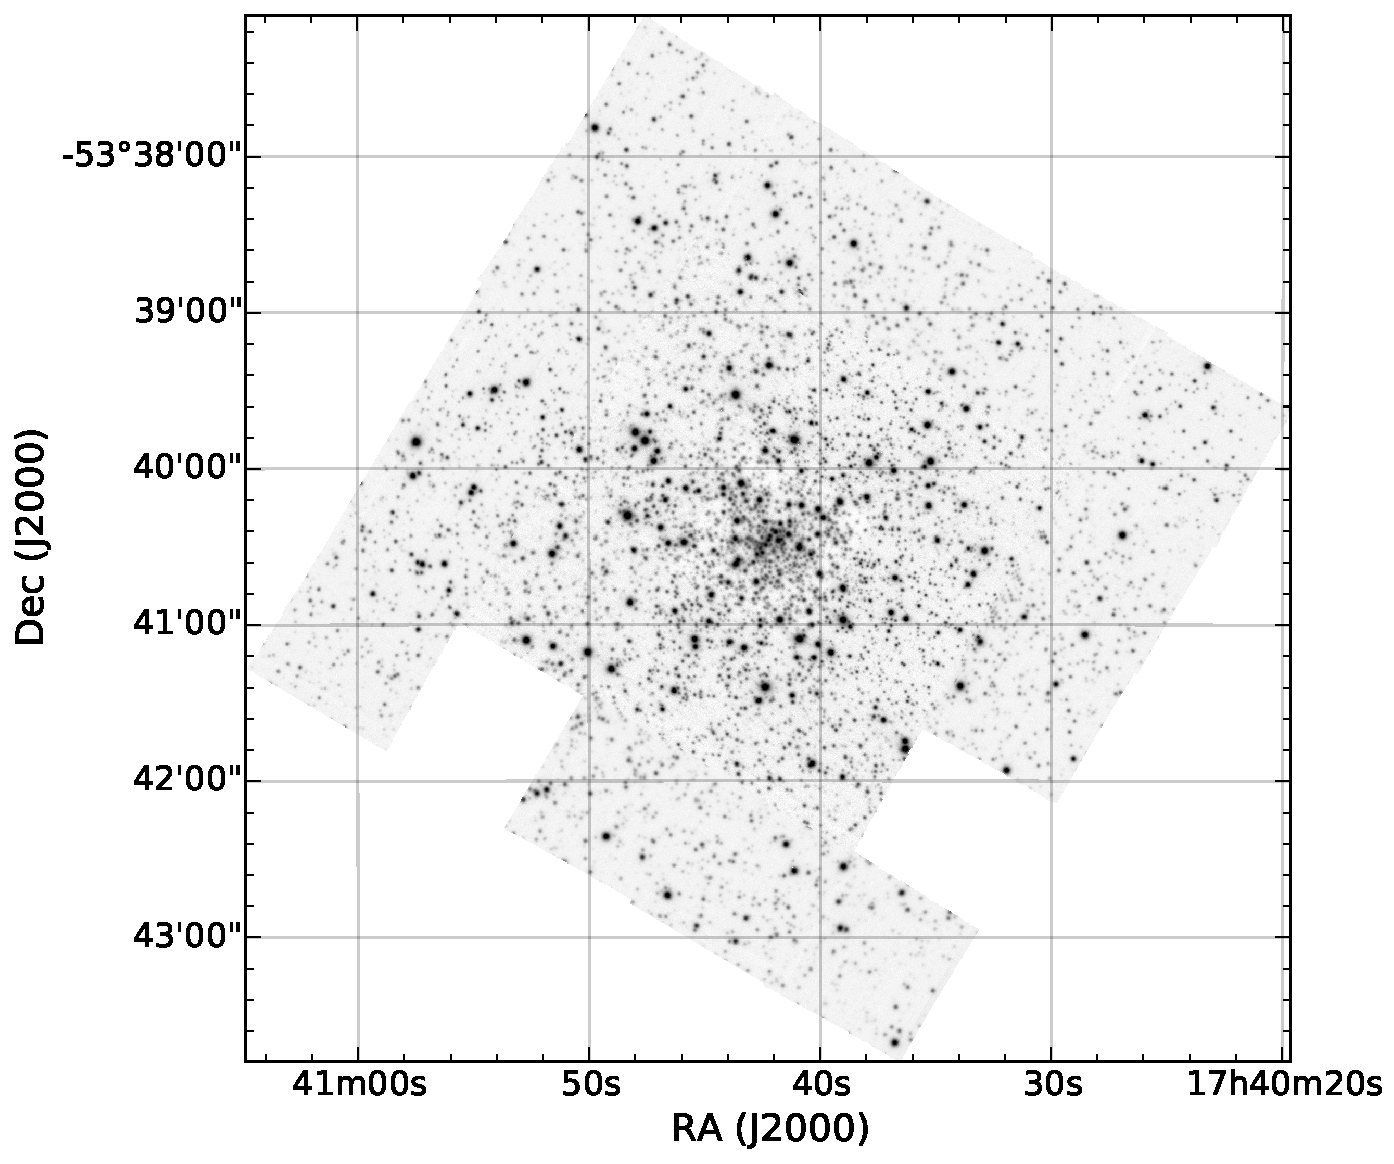
\includegraphics[scale=.6]{assets/images/mosaic.pdf}
\caption{White image mosaic of MUSE data cubes of NGC 6397. }
\label{fig:clustermuse}
\end{figure}

\section{Processed and Raw data} 

The primary goal of the MUSE observation of NGC 6397 was to create the first comprehensive Hertzsprung-Russell diagram with a sample of over 12000 spectra \citep{husser_muse_2016}. The large number of spectra obtained allowed them to study the kinematics of the globular cluster with the goal to probe the presence of a central black hole in the cluster \citep{kamann_muse_2016}. This data is publicly available thought the \emph{MUSE Science Web Service}\footnote{\url{http://muse-vlt.eu/science/}}. The website contains advanced science products such as reduced datacubes, source catalogs and software tools. For NGC 6397, the spectra of the stars in the globular cluster NGC 6397 as published in the studies mentioned above (\citealp{husser_muse_2016} and \citealp{kamann_muse_2016}) are provided. They provided all the obtained spectra with a signal-to-noise ratio of five or larger, i.e. 14 271 spectra in total. For our goal to study the CVs in the globular clusters the published spectra were not enough as they mainly cover the range from main sequence to the tip of the red giant branch\footnote{The red giant branch phase is the stage of stellar evolution that follows the main sequence for low to intermediate-mass stars. During this phase the stellar atmosphere expands and the helium core contracts. This phase precedes the Helium burning phase. }. Our approach in this project was to work with the raw science data. The science data can be obtained from the ESO  Science Archive Facility. As stated in the ESO Data Access Policy\footnote{\url{http://archive.eso.org/cms/eso-data-access-policy.html}}, all science data is made publicly available through the science archive after the proprietary period (normally one year after the data have been made available to the principal investigator) and all calibration data are public immediately after the observations.  

\subsection{Data Reduction}

I reduced the data with version 1.2.1 of the MUSE Instrument Pipeline Recipes\footnote{The MUSE pipeline can be found at \url{http://www.eso.org/sci/software/pipelines/muse/}}\citep{weilbacher_design_2012}. The pipeline distribution kit includes several packages. The ones used for this work are the following:

\begin{itemize}
        \item The Common Pipeline Library version 6.6 \citep{mckay_common_2004}
        \item The ESO Recipe Execution Tool (EsoRex)\footnote{EsoRex is written by the CPL group (Pipeline System Department) European Southern Observatory \url{http://www.eso.org/sci/software/cpl/esorex.html}} version 3.12.
\end{itemize}

All the data reduction was done calling \emph{EsoRex} to execute the MUSE DRS recipes from a bash (version 4.3.11) script\footnote{All the configuration files for each of the MUSE recipes used, the bash scripts I wrote, useful python (Python 2.7.6) scripts, the scripts and data for all the plots produced and other text files generated during this internship relevant for the data reduction can be found at \url{https://github.com/manuelmarcano22/muse2016}} (alternatively this can be done via the Python bindings, \cite{streicher_python_2012}). We summarize the main steps to produce the fully reduced data cube from the raw science and calibration data download from the ESO Science Archive MUSE Query Form. The data reduction steps can be divided into two categories, pre-processing and post-processing. The pre-processing includes all the necessary calibration to remove the instrument signature on the exposures. In the post-processing then the resulting pixel table for each science observation is calibrated for flux and astrometry, and then resampled into a data cube.

\begin{enumerate}
        \item Pre-processing
                \begin{enumerate}[I]
			\item \textbf{Bias subtraction}: Bias subtraction was done by combining 10 different bias images into one master bias file. The combination was done using the sigma clipping technique. Other possible options are combining using the median or average method. Each bias is part of the calibration files taken by ESO every night. A bias frame is dark image with no exposure time taken to account for the read out noise. (Recipe called \emph{muse\_bias}). For this and all subsequent steps we used a table of additional bad pixels of the CCDs created for the MUSE commission runs. This bad pixel table is distributed along with the MUSE pipeline files. 
            \item \textbf{Flat-fielding}: For the flat-field correction 10 individual flat frames were combined into a master flat frame (using the sigma clipping technique). The flat-field images are taking daily at the VLT as part of the standard calibration plan.  The master flat  contains  the  combined  pixel  values  of  the  raw  flat exposures. The purpose is to correct for uneven detector sensitivity. The recipe used was \emph{muse\_flat}. Besides the master flat, the recipe also produces a \emph{trace table} containing polynomials defining the location of the slices on the CCD. 
			\item \textbf{Wavelength calibration}: For the wavelength calibration, 15 different arc lamp exposures were used. These are 3 per lamp (Ne, Xe, HgCd lamps). The recipe used is \emph{muse\_wavecal}. It detects arc emission lines and determine the wavelength solution for each slice. The goal is to establish the pixel to wavelength equivalence with high precision.
			\item \textbf{Line Spread Function}: The line-spread function is calculated with the recipe \emph{muse\_lsf}. The lines spread function describes the broadening of spectral lines on a CCD. The recipe calculates this  wavelength dependent function from 15 arc lamp exposures, and the wavelength solution calculated in the step above.  
			\item \textbf{Geometrical calibration}: In this step, the recipe \emph{muse\_geometry} computes  relative  location  of the slices within the field of view and measures the instrumental point spread function on the detectors. This creates a geometry table. A geometry table comes with the standard MUSE pipeline package as a static calibration file. The geometry table prepared for the third commissioning period was used in reducing the data. 
			\item \textbf{Illumination Correction}: Flat-fields from the sky or twilight flats are taken weekly at the VLT. These are use to do large scale illumination correction. For the illumination correction also a special purpose  illumination flat field called ILLUM can be used as an input to the recipe. These are taken throughout the observing night. We use the one taken closest in time to the science data. Both twilight flats and the ILLUM were used as input to the recipe \emph{muse\_twilight}.
    
    \item{\textbf{Pixel table creation}}: This step removes all the instrumental signatures on the science exposures and converts them from an image to a large table (called a pixel-table). After calling the recipe \emph{muse\_scibasic}, for each science frame a pixel table is created. The recipe uses the calibration files produced before (master bias, master flat, geometry table, bad pixel table, twilight correction). These tables are the input frames in the subsequent post-processing phase.
    \end{enumerate}
\item Post-processing
                \begin{enumerate}[I]
			\item \textbf{Flux calibration}:  In this step a flux response curve from a standard star exposure is created. The end product of the \emph{muse\_standard} are tables with the response curve as derived from the standard star and the telluric absorption.
                        \item \textbf{Sky subtraction}: This step is only needed if the observed object fills the field of view. In the case of the NGC 6397 observation, a reasonable sky spectrum can be obtained on the observation itself and used to substract the sky.   
                        \item \textbf{Astrometry}: An astrometry solution was done by the MUSE consortium for the third commissioning period. The astrometry solution comes with the MUSE pipeline and was the one used for the data astrometry correction.  
          
                        \item \textbf{Cube assembly}: In this last part, a full data cube is created from a single exposure, the sky background is removed and the flux and the astrometric calibration are applied. In this step the cubes are sampled to a common value $(0\farcs 2 \times 0\farcs 2 \times 1.25 \text{ \r A})$. Individual data cubes from single exposures can be merged into a single data cube. This was done for each of the 23 different region of the cluster observed. For the center regions, data cubes for the individual exposures were also created.  
                \end{enumerate}
\end{enumerate}


\subsection{Spectral extraction and analysis}

The spectral subtraction and analysis was carried out with a number of open-source scientific software. To visualize the data cubes and extract the spectra for analysis, QFitsView\footnote{\url{http://www.mpe.mpg.de/~ott/QFitsView/}} was used. This is the graphical front-end written QT library of the DPUSER language. Spectral analysis and fitting was done with IRAF \citep{1986SPIE..627..733T} (mainly through the command language based on Python PyRAF\footnote{PyRAF is a product of the Space Telescope Science Institute operated for NASA by AURA}) and Astropy \citep{astropy_collaboration_2013}. To calculate magnitudes the package Astrolib PySynphot (pysynphot) from the Space Telescope Science Institute was used \citep{pysynphot} and for plotting we made use of the APLpy package, an open-source plotting package for Python hosted at http://aplpy.github.com

\begin{comment}
s images to form a master
bias, combine 5 lamp-flat exposures, and use one exposure
of each arc lamp to derive the wavelength solution. 11 skyflats,
taken during the evening twilight preceding the science exposures,
were combined and used to create a 3D correction of the
illumination in the range λ = 5000 . . . 8000 Å2
.
The geometry of the instrument was derived f

. These calibrations were found
to be valid for the full period of the first commissioning run of
the instrument and were also shipped with the MUSE pipeline.
i
Pix talbe
he di
erence between sky andnn
calibration unit illumination. The result of this process is a
large table (hereafter called a pixel-table) for each science frame. This table contains all pixel values corrected for bias and flat-field and their location on the detector. A geometri- cal calibration and the wavelength calibration solution were used to transform the detector coordinate positions to wave- lengths in Ångström and focal plane spatial coordinates 

\end{comment}
